\section{Proof of Concept Attacks}
The previous section (Section. \ref{Arch:Test}) discussed in detail how we verified that our system functions according to our expectations. This section details how we validated our expectations. In order to do this, we constructed 3 sets of web applications in PHP, Python, and Ruby. Each of these applications was a simple web app that took in user input to construct and send an E-Mail.

The front-end for each of the three applications is shown in Listing. \ref{code:html}. The back-end for the three languages are shown in Listings \ref{code:phpemi}, \ref{code:pyemi}, and \ref{code:rubyemi}.

We tested for the headers being injected in real-time by running an instance of MailCatcher, set to listen on all SMTP messages. A sample screenshot of a fuzzed request for the Ruby backend (generated in PostMan) is shown in Fig. \ref{fig:postmanruby}. The E-Mail sent due to injecting this payload (as captured by MailCatcher) is shown in Fig. \ref{fig:mailcatcherruby}. It can be seen that the Headers have been added to the resulting E-Mail, and we have successfully managed to overwrite the `Subject' field with our own message.\\
Both PHP and Python are injected with headers in a similar way.

\lstset{language=HTML,caption={E-Mail Header Injection - Front-End},label={code:html}}
\begin{lstlisting}
<!doctype html>
<html lang="en">
<head>
<meta charset="utf-8">
<meta http-equiv="x-ua-compatible" content="ie=edge">
<title>Mock Email</title>
<meta name="author" content="Sai Pc">
<meta name="viewport" content="width=device-width, initial-scale=1">
</head>
<body>
<div id="container" class="container">
<form action="{Replace with path to back-end}" method="post">
<input type="text" placeholder="Email" name="email" id="email"><br>
<textarea name="msg" rows="120" cols="20"></textarea>
<input type="submit" value="Email Me!!">
</form>
</div>
</body>
</html>

\end{lstlisting}

\begin{figure}[!htbp]
	\centering
	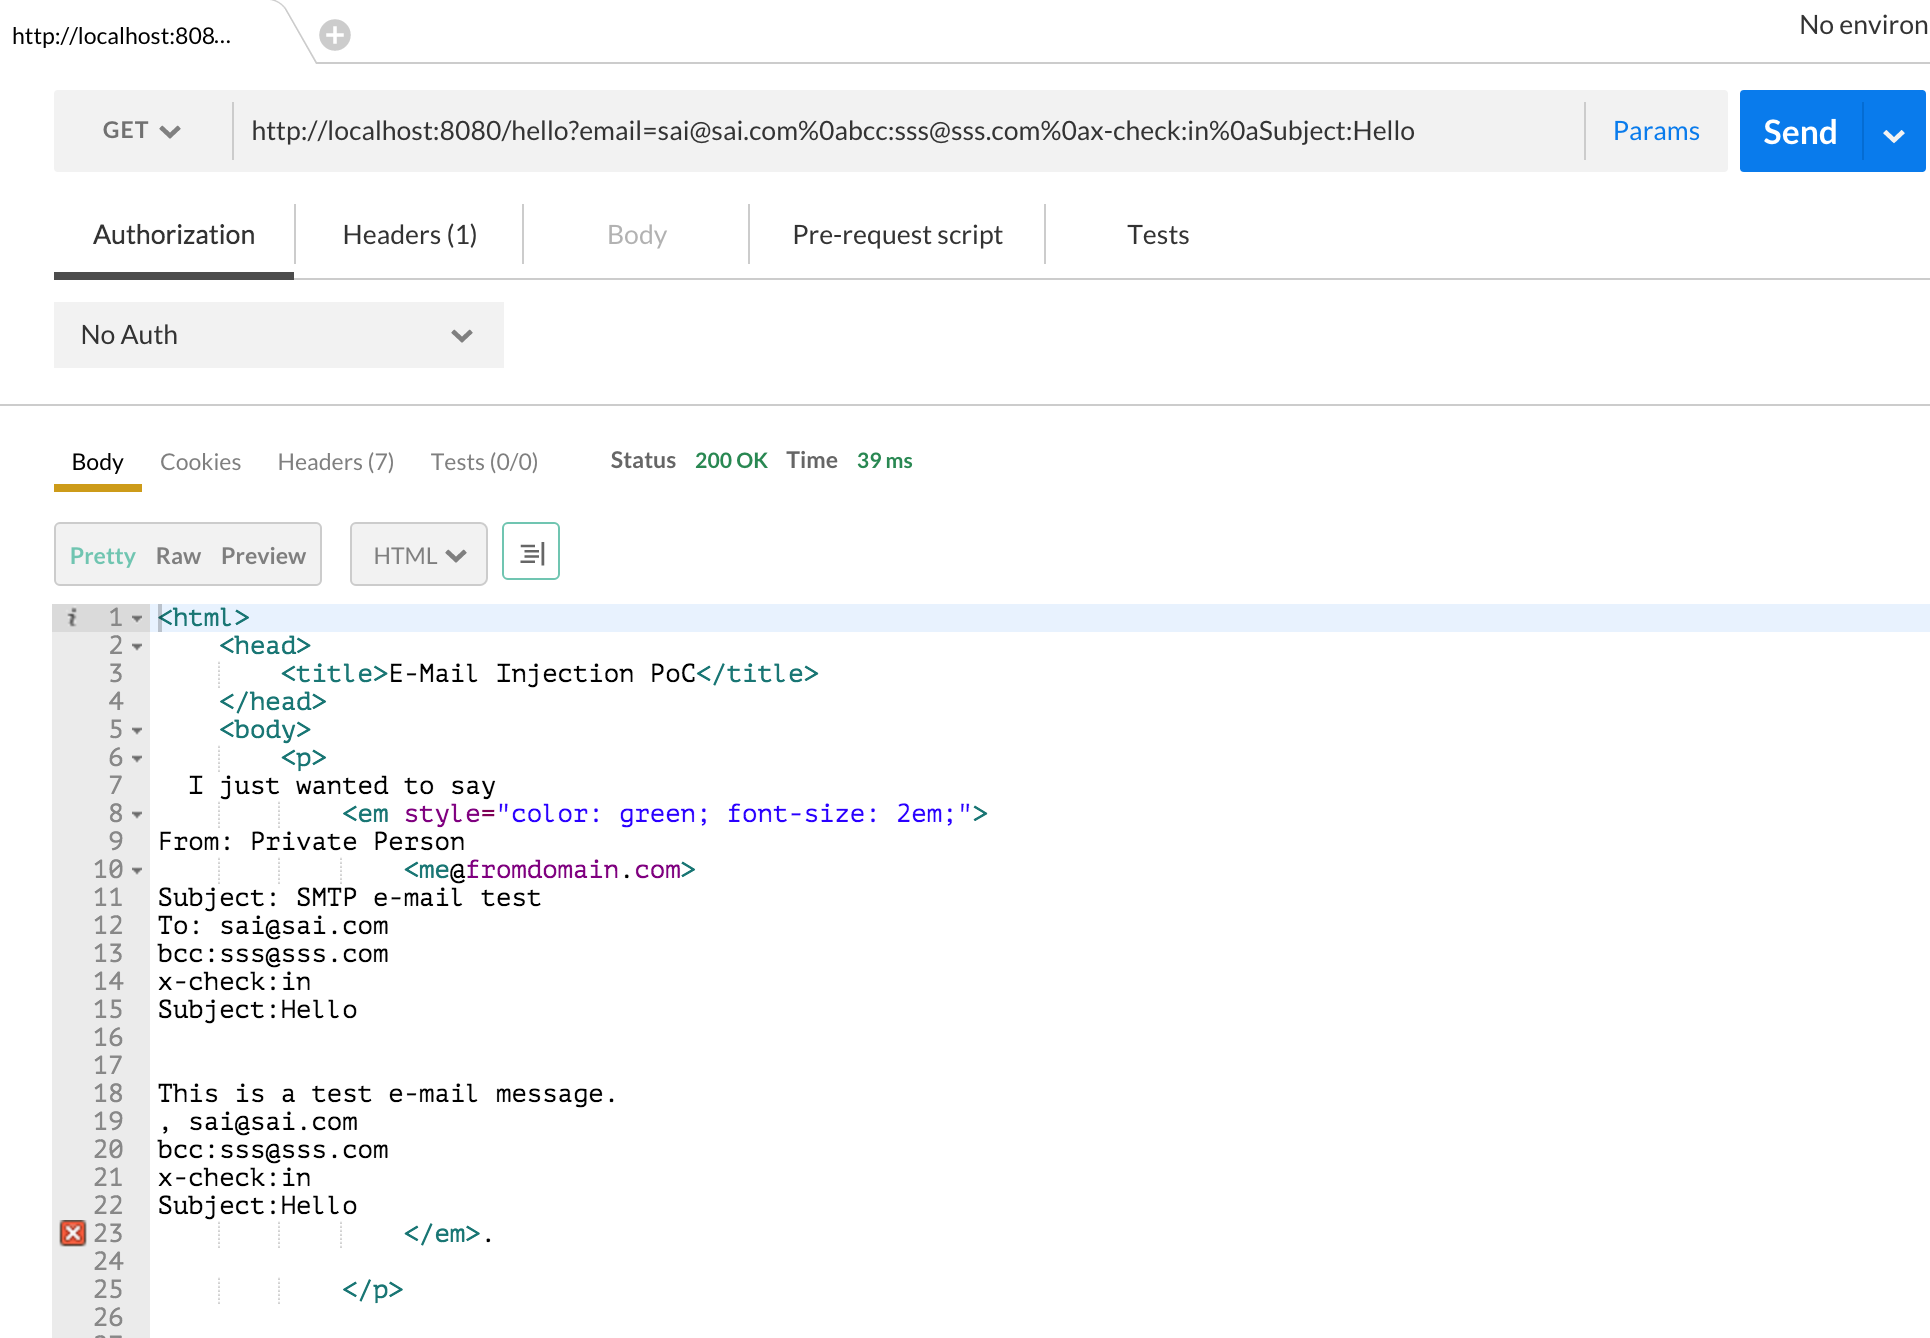
\includegraphics[width=14cm, height=9cm]{System/EMI_Postman_Ruby}
	\caption{Fuzzed Request for Ruby}
	\label{fig:postmanruby}
\end{figure}

\begin{figure}[!htbp]
	\centering
	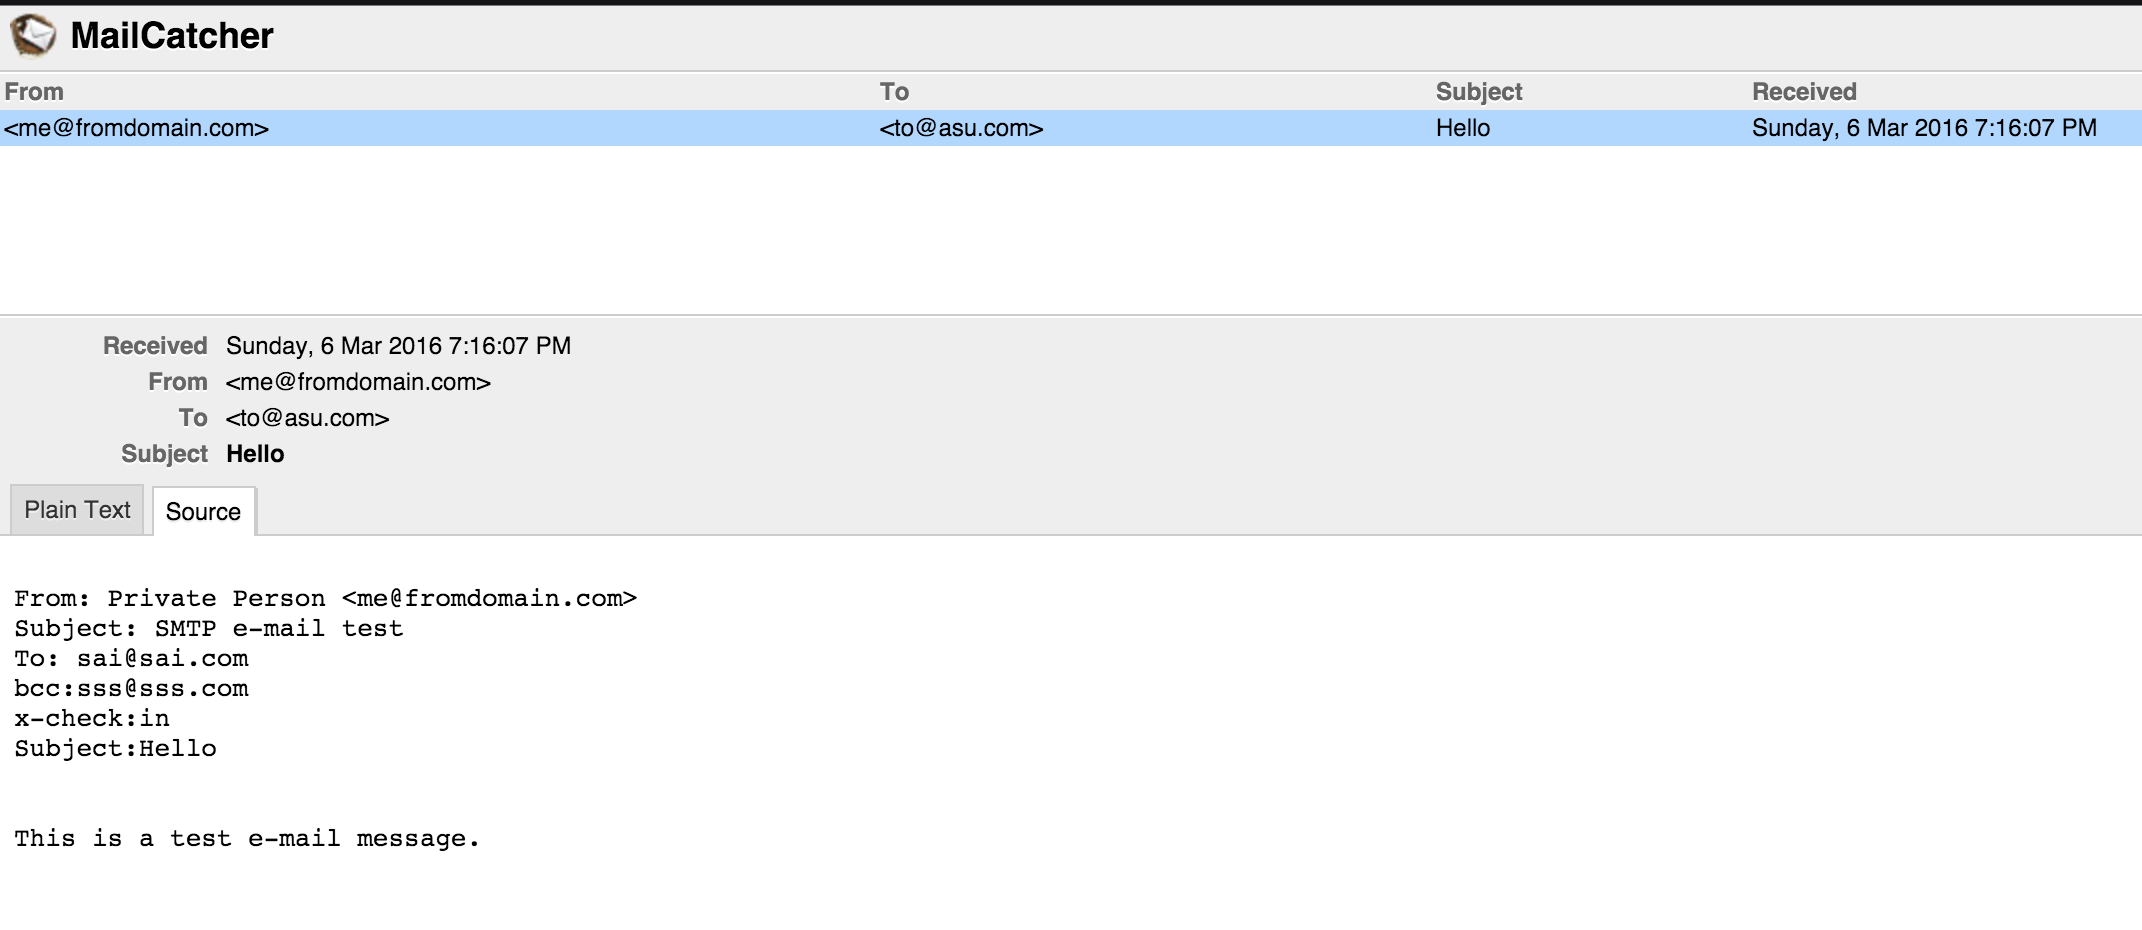
\includegraphics[width=14cm, height=9cm]{System/EMI_Mailcatcher_Ruby}
	\caption{E-Mail Header Injection Proof of Concept - Ruby}
	\label{fig:mailcatcherruby}
\end{figure}